\begin{problem}{전생했더니 슬라임 연구자였던 건에 대하여 (Hard)}{standard input}{standard output}

안녕? 내 이름은 ntopia!

나는 원래 지구에 살고 있던 평범한 20대 청년이었어. 어느 날 길을 걷다가 괴한의 칼에 찔려
죽어버렸어. 그런데 이게 무슨 일이람! 정신을 차려보니 이i세계에 떨어져 버렸지 뭐야.
여기에서 나는 슬라임을 전문으로 연구하는 슬라임 연구자가 되어버린 것 같아.
나는 지금 아주 중요한 연구를 진행하고 있어. 이 연구가 성공하면 나는 내가 살던 세계로
돌아갈 수 있게 될 거야. 이 연구를 도와주지 않겠니?

이곳의 슬라임은 모두 슬라임 에너지라는 것을 갖고 있고 그 양은 2 이상의 자연수로 표현돼.
나는 슬라임을 합성했을 때 슬라임 에너지가 어떻게 변화하는지에 대해 연구하고 있어.

슬라임 합성 과정은 2마리를 합성해서 1마리를 만들어내는 식으로 이루어져.
$A$만큼의 슬라임 에너지를 가진 슬라임과 $B$만큼의 슬라임 에너지를 갖고 있는
슬라임이 있었다고 해보자. 이 슬라임 2마리를 합성하면
슬라임 에너지가 $A \times B$ 인 슬라임을 만들 수 있어.

그리고 슬라임 합성 기술이 아직 완벽하지 않아서 슬라임을 합성할 때마다
크나큰 전기 에너지가 필요해. 구체적으로,
$A$만큼의 슬라임 에너지를 가진 슬라임과 $B$만큼의 슬라임 에너지를 가진 슬라임을
합성하려면 $A \times B$ 만큼의 전기 에너지가 필요해.

\begin{center}
  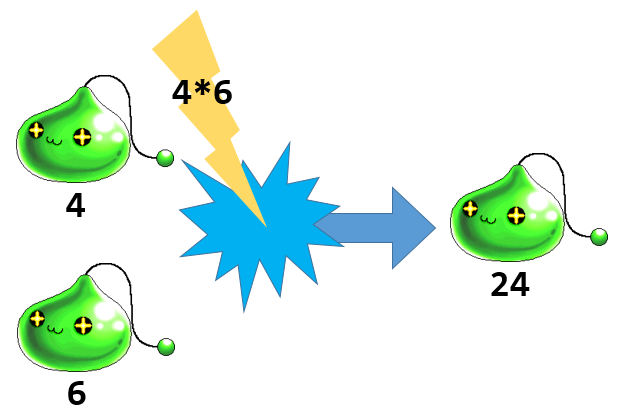
\includegraphics[width=0.7\textwidth]{slime_compose.png}
  \begin{figure}[!h]
  \captionsetup{labelformat=empty,justification=centering}
  \caption{에너지가 $4$인 슬라임과 에너지가 $6$인 슬라임을 합성한 모습. $4\times6$의 전기 에너지를 사용해 슬라임 에너지가 $24$인 슬라임이 합성되었다.}
  \end{figure}
\end{center}

나에겐 지금 $N$마리의 슬라임이 있어. 이 슬라임들을 모두 적절히 합성해서
1마리의 슬라임으로 만들려고 해. 그런데 내가 소속된 연구소에서
각 합성 단계마다 필요한 전기 에너지들을 모두 곱한 값을 나에게 비용으로
청구하겠다고 했지 뭐야. 그래서 이 값이 최소가 되도록 합성을 적절히 수행하는 것이 내 연구의 목표야.

내 연구를 도와줘! 부탁이야!!

\InputFile
첫 번째 줄에 테스트 케이스의 수 $T$ 가 주어지고, 이어서 $T$ 개의 테스트 케이스가 주어진다.

각 테스트 케이스의 첫 번째 줄에는 슬라임의 수 $N$ ($1 \le N \le 60$)이 주어지고, 두 번째 줄에는 $N$ 개의 자연수가 주어진다. $i$번째 자연수 $C_i$ ($2 \le C_i \le 2 \times 10^{18}$) 는 $i$번째 슬라임의 슬라임 에너지를 나타낸다. 끝까지 합성하고 난 후에 생기는 슬라임의 에너지의 양이 $2 \times 10^{18}$ 이하라는 것이 보장된다.

모든 테스트 케이스에 대한 $N$ 의 총합이 $1,000,000$을 넘지 않음이 보장된다.

\OutputFile
각 테스트 케이스마다 슬라임을 끝까지 합성했을 때 청구될 비용의 최솟값을 $1,000,000,007$로 나눈 나머지를 출력한다.
전기 에너지가 전혀 필요하지 않은 경우엔 $1$ 을 출력한다.

\Example

\begin{example}
\exmp{2
5
3 10 2 8 14
1
13}{270950400
1}%
\end{example}

\end{problem}
